\documentclass[10pt]{beamer}
\def\*#1{\mathbf{#1}}
\def\ab{ab}

\usetheme{metropolis}
\usepackage{appendixnumberbeamer}

\usepackage{booktabs}
\usepackage[scale=2]{ccicons}

\usepackage{pgfplots}
\usepgfplotslibrary{dateplot}

\usepackage{xspace}
\newcommand{\themename}{\textbf{\textsc{metropolis}}\xspace}

\title{Quesion Answering}
\subtitle{CS671: Course Project}
\date{\today}
\author{}
\institute{}

\setbeamercolor{alerted text}{fg=black}

\begin{document}

\maketitle

% \begin{frame}{Table of contents}
%   \setbeamertemplate{section in toc}[sections numbered]
%   \tableofcontents[hideallsubsections]
% \end{frame}

\section{Dataset}

\begin{frame}[fragile]{SQuAD Dataset}

	\begin{itemize}[<+- | alert@+>]
		\item Stanford Question Answering Dataset (SQuAD) is a reading comprehension dataset, consisting of questions posed by crowdworkers on a set of Wikipedia articles, where the answer to every question is a segment of text, or span, from the corresponding reading context.
		\item  The training set consists of around 100,000+ question-answer pairs on 500+ wikipedia articles
	\end{itemize}
\end{frame}

\begin{frame}[fragile]{SQuAD Dataset Example}

	\begin{itemize}[<+- | alert@+>]
		\item \textbf{Context : } "The Joan B. Kroc Institute for International Peace Studies at the University of Notre Dame is dedicated to research, education and outreach on the causes of violent conflict and the conditions for sustainable peace. It offers PhD, Master's, and undergraduate degrees in peace studies. It was founded in 1986 through the donations of Joan B. Kroc, the widow of McDonald's owner Ray Kroc. The institute was inspired by the vision of the Rev. Theodore M. Hesburgh CSC, President Emeritus of the University of Notre Dame. The institute has contributed to international policy discussions about peace building practices."
		\item  \textbf{Question : } "What institute at Notre Dame studies  the reasons for violent conflict?"
		\item \textbf{Answer : } "Joan B. Kroc Institute for International Peace Studies"
		\item \textbf{Answer Start : } 4
	\end{itemize}
\end{frame}

\begin{frame}[fragile]{Analysing SQuAD Dataset}

	\begin{itemize}[<+- | alert@+>]
		\item Answer to the SQuAD questions are directly drawn from text, so any model need to predict only correct starting and ending point to answer rather than producing any texts.
		\item We perform some basic analysis on the dataset in the form of histograms
			of the context paragraph lengths,  question lengths,  and answer lengths in the training set.
	\end{itemize}
\end{frame}

\begin{frame}[fragile]{Analysing SQuAD Dataset - Graph(1/4)}

	\begin{figure}[H]
		\centering
		{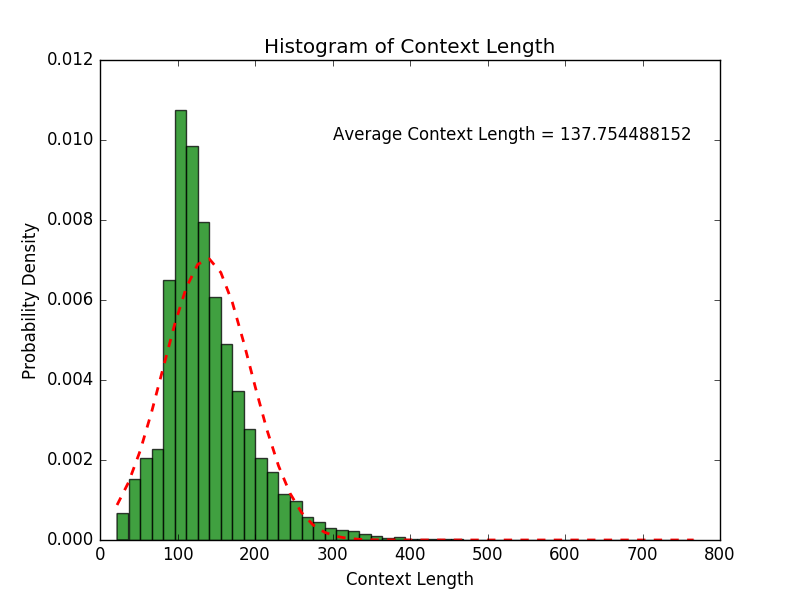
\includegraphics[width=0.8\textwidth]{context_hist_fin.png}\label{fig:f1}}
%   \caption{Histogram of Context Paragraph Lengths}
	\end{figure}

	\begin{itemize}
		\item As we can easily see, most paragraphs do not exceed 300 words.
	\end{itemize}
\end{frame}

\begin{frame}[fragile]{Analysing SQuAD Dataset - Graph(2/4)}

	\begin{figure}[H]
		\centering
		{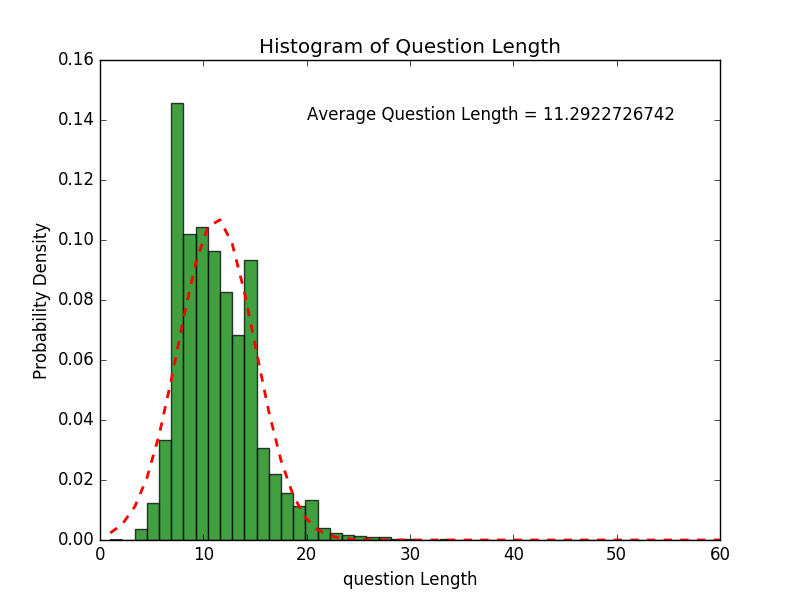
\includegraphics[width=0.8\textwidth]{question_hist_fin.png}\label{fig:f1}}
%   \caption{Histogram of Question Lengths}
	\end{figure}

	\begin{itemize}
		\item Almost no question longer than 30 words.
	\end{itemize}
\end{frame}

\begin{frame}[fragile]{Analysing SQuAD Dataset - Graph(3/4)}

	\begin{figure}[H]
		\centering
		{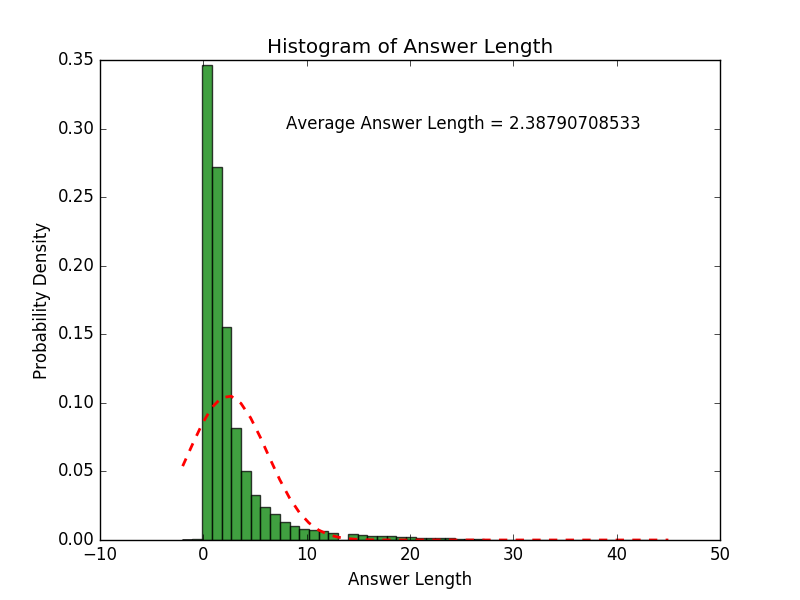
\includegraphics[width=0.7\textwidth]{ans_hist_fin.png}\label{fig:f1}}
%   \caption{Histogram of Context Paragraph Length}
	\end{figure}

	\begin{itemize}
		\item Most answers
			are shorter than 10 words.
	\end{itemize}
\end{frame}

\begin{frame}[fragile]{Analysing SQuAD Dataset - Graph(4/4)}

	\begin{figure}[H]
		\centering
		{\includegraphics[width=0.9\textwidth]{dist.png}\label{fig:f1}}
%   \caption{Histogram of Context Paragraph Length}
	\end{figure}
\end{frame}

\begin{frame}[fragile]{Analysing SQuAD Dataset}

	\begin{itemize}
		\item Based on the above analysis, we set an optimal choice for hyper parameters such as maxContextLength, maxQuestionLength, maxAnswerLength and use these to clip / pad the contexts, questions and answers
	\end{itemize}
\end{frame}

\begin{frame}[fragile]{Models}

	We explore two models for the machine comprehension task,
	\pause
	\begin{itemize}[<+- | @alert->]
		\item Match-LSTM and Answer Pointer
		\item Bidaf
	\end{itemize}
\end{frame}

\section{Match-LSTM and Answer Pointer}

\begin{frame}[fragile]{LSTM Preprocessing Layer}

	\begin{itemize}[<+- | alert@+>]
		\item The purpose of the \et{LSTM Preprocessing Layer} is to incorporate contextual information into the representation of each token in the context and the question.
		\item \begin{align*}
				\boldsymbol{H}^p = \overrightarrow{\text{LSTM}}(\boldsymbol{P}), \quad\quad
				\boldsymbol{H}^q	=	\overrightarrow{\text{LSTM}}(\boldsymbol{Q})
			\end{align*}
		\item The matrices $\boldsymbol{H}^p$ and $\boldsymbol{H}^q$ represent the hidden representations of the context and the question matrices, respectively.
	\end{itemize}
\end{frame}

\begin{frame}{Match-LSTM Layer}
	\begin{itemize}[<+- | alert@+>]
		\item Question is treated as a premise and answer as a hypothesis
		\item The match-LSTM sequentially goes through the context.
		\item At position $i$ the word-by-word attention is calculated as follows:
		\item
			\begin{align*}
				\boldsymbol{G_i} &= tanh(\*W^q\*H^q + (\*W^p\*h_i^p+\*W^r\*h_{i-1}^r+\*b^p)\otimes e_{\*Q})\\
				\overrightarrow{\alpha_i} & = softmax(\*w^T\overrightarrow{\*G_i}+b\otimes\*e_Q)
			\end{align*}
		\item where $\*W^q$, $\*W^p$, $\*W^r$, $\in$ $\mathbb{R}^{l\times l}$, $\*b,\*w \in \mathbb{R}^l$ and $\*b \in \mathbb{R}$ are the parameters to be learned.
		\item $\overrightarrow{\*h_{i-1}^{r}} \in \mathbb{R}^l$ is the hidden vector at position i-1
	\end{itemize}
\end{frame}

\begin{frame}{Match-LSTM Layer}
	\begin{itemize}[<+- | alert@+>]
		\item Take the weighted version of the question and combine it with the current token of the context to form a vector $\overrightarrow{\*z_i}$:
			$$\overrightarrow{z_i} =
			\begin{bmatrix}
				\*h_i^p \\ \*H^q\overrightarrow{\alpha_i}^T
			\end{bmatrix}
			$$
		\item This vector $\overrightarrow{\*z_i}$ is fed into a standard one-directional LSTM to form our so-called match-LSTM:
			$$\overrightarrow{\*h_i^r} = \overrightarrow{\text{LSTM}}(\overrightarrow{\*z_i},\overrightarrow{\*h_{i-1}^r}),$$
			where $\overrightarrow{\*h_i^r}\in \mathbb{R}^l$
	\end{itemize}
\end{frame}

\begin{frame}{Match-LSTM Layer}
	\begin{itemize}[<+- | alert@+>]
		\item Similar Match-LSTM layer is build in the reverse direction.
		\item Obtain a representation that encodes the contexts from both directions for each token in the context
		\item
			\begin{align*}
				\overleftarrow{\*G_i} &= tanh(\*W^q\*H^q + (\*W^p\*h_i^p + \*W^r\overleftarrow{h}_{i+1}^r\*b^p)\otimes \*e_Q),\\
				\overleftarrow{\alpha_i} & = softmax(\*w^T\overleftarrow{\*G_i}+b\otimes \*e_Q),
			\end{align*}
			where the parameters are $(\*W^q,\*W^p,\*W^r,\*b^p,\*w \ and \ b)$
		\item $\*z_i$ and $\*h_i$ are defined in similar manner.
	\end{itemize}
\end{frame}

\begin{frame}{Match-LSTM Layer}

	\begin{itemize}[<+- | alert@+>]
		\item $\overrightarrow{\*H^r} \in \mathbb{R}^{l\times P}$represents the hidden states $[\overrightarrow{\*h_1^r},\dots,\overrightarrow{\*h_P^r}]$
		\item Similarly $\overleftarrow{\*H^r}\in \mathbb{R}^{l\times P}$ represents $[\overleftarrow{\*h_1^r},\dots,\overleftarrow{\*h_P^r}]$
		\item $\*H^r \in \mathbb{R}^{2l \times P}$ as
			$$\*H^r = \begin{bmatrix}
				\overrightarrow{\*H^r}\\ \overleftarrow{H^r}
			\end{bmatrix}$$
	\end{itemize}

\end{frame}

\begin{frame}{Answer Pointer Layerd}
	\begin{itemize}[<+- | alert@+>]
		\item The model takes $\*H^r$ as input and tries to predict the answer.
		\item \textbf{Boundary Model}: Concerned with the starting and ending tokens of the answer.
		\item The probability of answer is modelled as $$\mathbb{P}[\*a|\*H^r] = \mathbb{p}[a_s|\*H^r]\mathbb{P}[a_e|a_s,\*H^r]$$
		\item This is used to compute a \textbf{attention vector} $\*\beta_k \in \mathbb{R}^{P+1}$, where $\beta_{j, k}$ is the probability of selecting the $j$\tth context token as the $k$\tth token in the answer.
			$$\mathbb{P}[a_k = j| a_1, a_2 \dots a_{k - 1}, \*H^r] =	\beta_{j, k}$$
		\item Objective is to maximize $\mathbb{P}[\*a|\*H^r]$, and the answer corresponding to the maximum answer is reported as the answer to the query
	\end{itemize}

\end{frame}

\begin{frame}{Answer Pointer Layer}
	\begin{itemize}[<+- | alert@+>]
		\item The answer pointer does not differentiate the question types, and therefore all questions - what? where? why? how? etc. will be answered using the same attention mechanism
		\item In order to differentiate, we setup different Answer Pointer layers for different question types
		\item This allows us to model each question type differently
	\end{itemize}
\end{frame}

\begin{frame}{Loss Function}

	\begin{itemize}[<+- | alert@+>]
		\item The loss function for the Answer Pointer Layer is the Sigmoidal Cross-Entropy Loss
		\item For each answer token, the cross entropy is computed and added to the total loss
		\item For the boundary model, there are only two answer tokens, the start and the end
		\item The loss is given as 
			\begin{align*}
				- \log{p(a_s \,|\, \boldsymbol{P}_n, \boldsymbol{Q}_n)} - \log{p(a_e \,|\, \boldsymbol{P}_n, \boldsymbol{Q}_n)}
			\end{align*}
	\end{itemize}

\end{frame}

\begin{frame}{Weighted Loss}
	
\end{frame}

\section{Attention}
\begin{frame}{Attention}
	\begin{itemize}
		\item Model learns what to attend based on the input query.
		\item Mapping a query and a set of key-value pairs to an output.
		\item Output is a weighted sum of the values, weights are computed by a compatibility function of the query with the corresponding key.
	\end{itemize}

\end{frame}

\subsection{Scaled Dot-Product Attention}

\begin{frame}{Scaled Dot-Product Attention}
	\begin{figure}[ht!]
		\centering
		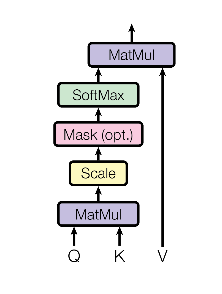
\includegraphics[height=100px]{Attention-Dot.png}
		\caption{Scaled Dot-Product Attention \et{\citep[Source:][]{--Attention is all you need}}}
		\label{fig:dot-attention}
	\end{figure}
	\vspace{-20}
	\begin{itemize}
		\item We compute the dot products of the
			query($d_k$) with all keys($d_k$).
		\item Attention function is calculated on a set of queries simultaneously, packed together into a matrix Q.
		\item The keys and values are packed together into matrices K and V.
	\end{itemize}

\end{frame}
\begin{frame}{Scaled Dot-Product Attention}
	\begin{center}
		\[
			\text{Attention}(Q, K, V) = softmax(\frac{QK^{T}}{\sqrt{d_k}}) V
		\]
	\end{center}
	\begin{itemize}
		\item For large values of $d_k$ , the dot products grow large in magnitude. pushing the softmax function into regions where it has extremely small gradients. To counteract this effect, dot product is scaled by $\frac{1}{\sqrt{d}}$ .
		\item Dot-Product Attention is much faster and more space-efficient in practice as compared to additive attention.
	\end{itemize}
\end{frame}
\subsection{Multi-Head Attention}

\begin{frame}{Multi-Head Attention}
	\begin{figure}[ht!]
		\centering
		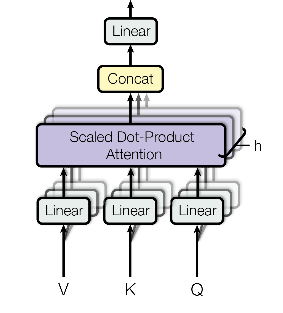
\includegraphics[height=100px]{Attention-Multi.png}
		\caption{Multi-Head Attention \et{\citep[Source:][]{--Attention is all you need}}}
		\label{fig:multi-attention}
	\end{figure}
	\vspace{-20}
	\begin{itemize}
		\item Linearly projecting the queries, keys and values h times with different, learned linear projections to $d_k$ , $d_k$ and $d_v$ dimensions, respectively.
		\item Now on each of these projected version perform the attention function in parallel.
	\end{itemize}
\end{frame}

\begin{frame}{Multi-Head Attention}
	\begin{center}
		\[
			\text {MultiHead}(Q, K, V) = Concat(head_1, ...,head_h)W^O\\
			where head_i = \text{Attention}(QW_i^Q, KW_i^K,VW_i^V)
		\]
	\end{center}
	Projection are parameter matrices $W_i^Q \in \mathbb{R}^{d_{model} \times d_k}, W_i^V \in \mathbb{R}^{d_{model}\times d_k}, W_i^Q \in \mathbb{R}^{d_{model} \times d_v}, W^O \in R^{{hd^v} \times d_mod}  $\\
	Due to the reduced dimension of each head, the total computational cost is similar to that of single-head attention with full dimensionality.
\end{frame}
\section{Pointer-Net}
\begin{frame}{Pointer Net}
	\begin{itemize}
		\item Used to predict the start(s) and end(e)
		\item Given the context representation $\{h_t^P\}_{t = 1}^n$, the attention mechanism is utilized as a pointer to select the start position ($p^1$ ) and end position ($p^2 $) from the context.
		\item
	\end{itemize}

\end{frame}
\section{Dynamic Programming}
\begin{frame}{Dynamic Programming}
	\begin{itemize}
		\item After getting the logits for start and end positions, Dynamic Programming strategies are used.
		\item We select $(s, e)$ where $s \leq e$ with the maximum value of $p_s^1p_e^2$, which can be calculated in linear time using dynamic programming.
		\item Legal answer is selected with highest join probability of start and end. The F1 score was improved by 2 points.
		\item We then used a sentence-level DP to find the maximum $p_s^1p_e^2$ where $s$ and $e$ are in same sentence. This improvement boosted the F1 score by another 0.5 point.
	\end{itemize}
\end{frame}

\end{document}
